% Order Shouldn't Matter: paper source, five-page main text plus a supplement.
% Self-contained: compiles with pdflatex + bibtex on a standard TeX Live. For an ACL submission replace the
% first four lines with \documentclass[11pt]{article} \usepackage[final]{acl} and drop geometry/titling;
% everything below the preamble is template-neutral. Tables under tables/ and figures under figures/ are
% generated by build.sh from paper/data/summary.json, which extract.py builds from the result files.
\documentclass[10pt,twocolumn]{article}
\usepackage[a4paper,margin=20mm,columnsep=7mm]{geometry}
\usepackage[T1]{fontenc}
\usepackage[utf8]{inputenc}
\usepackage{lmodern}
\usepackage{microtype}
\usepackage{graphicx}
\usepackage{booktabs}
\usepackage{natbib}
\usepackage{url}
\usepackage{amsmath}
\usepackage[hidelinks]{hyperref}
\hypersetup{pdftitle={Order Shouldn't Matter: What Disagreement Across Option Orders Adds Beyond the Averaged Confidence},
  pdfauthor={Erik Wistrand}, pdfsubject={Option-order sensitivity of first-token decision readouts from small language models},
  pdfkeywords={language models, multiple choice, option order, selection bias, uncertainty, calibration}}
\setlength{\bibsep}{2pt}
\renewcommand{\bibfont}{\small}
\setlength{\tabcolsep}{4pt}
\setcitestyle{authoryear,round}
\raggedbottom

\title{Order Shouldn't Matter: What Disagreement Across Option Orders Adds Beyond the Averaged Confidence}
\author{Erik Wistrand\\ \texttt{llav}, \url{https://github.com/wistrand/llav}}
\date{September 2026, draft}

\begin{document}
\maketitle

\begin{abstract}
Letter-probability readouts let a language model choose among named options without generating text, but the answer can depend on the options' arbitrary display order. Prior work shows that averaging over permuted orders mitigates the bias and that disagreement between orders can signal uncertainty. We ask whether that disagreement contributes anything once the reordered probabilities have been averaged, for multi-option decisions whose criteria and options are written at request time. On seven open models and 6,944 such decisions, asked in a randomized base order and up to six further distinct orders, the top choice changes on 24 to 60\% of questions; averaging after mapping probabilities back to the option identities reduces wrong answers by 5 to 21\% on every model and, as ensembling predicts, lowers the divergence from ChaosNLI's 100-annotator distributions. Added to the averaged answer's confidence in a held-out logistic combination, the continuous spread across orders gives no measurable error-ranking improvement (AUROC change $-0.0034$ to $+0.0007$). A change of top choice helps under this evaluation only when the base-order answer is kept, where it marks a subgroup with 1.8 to 4.1 times the adjusted error risk; after averaging it adds at most 0.0035 AUROC, and six of seven models decline. Under the tested combination and protocol, a system that pays for several orders gains nothing measurable from a second uncertainty feature built on their disagreement.
\end{abstract}

\section{Introduction}

Software increasingly asks language models structured questions with fixed answer types instead of asking for text: which team should handle this ticket, is this comment a personal attack, how frustrated is this customer on a three-point scale. One way to answer such a question is to read the model's next-token probabilities rather than generate text. The options are assigned letters, the prompt is evaluated once, and the probabilities of those letters are normalized over the option set \citep{semif2026,llav2026}. This produces one probability per option without generated text to parse.

The order of the options is an arbitrary choice the caller makes, and the model's answer depends on it. Suppose a router chooses between \emph{billing} and \emph{sales}. Listed as A: billing, B: sales, the model puts 0.55 on A and 0.45 on B. Listed the other way round, it puts 0.52 on A, which is now sales, and 0.48 on B. Mapped back to the option names, the two readings are billing 0.55 and 0.48: the top choice has changed, though nothing about the question has. Averaging the two aligned distributions gives billing 0.515 and sales 0.485. We call the size of the movement between the readings the \emph{spread} and a change of top choice a \emph{flip}; the top probability after normalizing over the options is the answer's \emph{confidence}, a score rather than a calibrated probability of being right.

Order sensitivity is known for benchmark multiple-choice questions, and averaging over permuted orders is the established mitigation \citep{pezeshkpour2024order,zheng2024robust,guda2025rethinking}; agreement between two orders is likewise an established reliability signal for pairwise judging \citep{scope2026}. We study decisions whose criteria and options are defined at request time, where there is no training set and the options are often near-synonyms written by the caller, and we ask a question the mitigation literature leaves open: once several orders have been evaluated and averaged, does their disagreement add error information beyond the confidence of the averaged answer? Across seven open models and 6,944 decisions, averaging reduces error on all seven models, and disagreement, continuous or discrete, does not improve error ranking once the orders are averaged. A flip does mark a higher-risk subgroup when a single order's answer is kept, so the answer depends on which answer a system retains.

\section{Experiment}
\label{sec:setting}

\begin{figure*}[t]
\centering
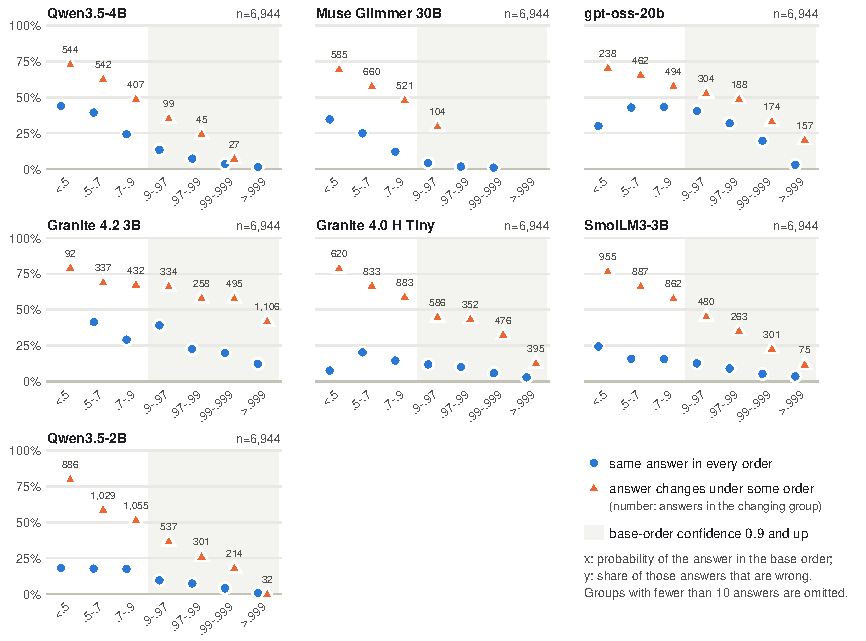
\includegraphics[width=\textwidth]{figures/fig1-bands.pdf}
\caption{Wrong-answer rate by the confidence of the answer in the base order, for answers whose top choice is the same in every order of the fixed budget (circles) and answers whose top choice changes (triangles, with the group's size). One panel per model, 6,944 questions each; groups with fewer than ten answers are omitted; the tinted region is the confident range the flag is used in. The changing group has the higher error rate in every band with enough answers, on every model, except Qwen 2B above 0.999.}
\label{fig:bands}
\end{figure*}

\paragraph{Readout.} A request carries a \emph{state} (the text) and a \texttt{choice} question that asks the model to select one of $n$ named, described options. The prompt is a fixed instruction (``Choose exactly one listed option. Respond with only its uppercase letter'') followed by a JSON payload. The payload holds the state, the criterion and the options as letters A to Z in the order given; it is SemIf's \texttt{direct-options-v1} prompt byte for byte \citep{semif2026}. Model reasoning modes are disabled. The model runs once through llama.cpp's server \citep{llamacpp}; the log-probabilities of the letters at the next token are softmaxed over the declared options and mapped back to the option names.

% The page break keeps the Orders paragraph from being split around Figure 1, which floats to the top of page 2.
\newpage
\paragraph{Orders.} Every question is asked in a \emph{base order} drawn at random per question, so a dataset's own option order is never the reference, and in six further random permutations, distinct from the base order and from one another. This \emph{fixed budget} is seven distinct orders for a question with four or more options and every distinct order for one with fewer (six for three options, two for two). Repeating an identical prompt changes no answer on three of the five models it was tried on and 0.5 to 0.6\% of answers on the other two. The mean spread between repeats is at most 0.003, compared with 0.10 to 0.25 between permutations, so repeat instability is too small to explain the effects below (Supplement~\ref{app:noise}).

\paragraph{Signals and targets.} The base order supplies its confidence. The fixed budget supplies the \emph{averaged} distribution's confidence, the \emph{spread}, which is the mean total-variation distance of each order's distribution from the average, and the \emph{flip}, whether the top choice differs across the orders. Two errors matter: whether the base-order answer is wrong (the single-order error) and whether the averaged answer is wrong. Error ranking is measured by AUROC, the probability that a score ranks a wrong answer as riskier than a right one (0.5 chance, 1.0 perfect).

\paragraph{Data and models.} The 6,944 choice questions come from ten source subsets. Each item's text forms the state, and the source's labels, with short descriptions, form the options. The ten subsets are AG News, DBpedia, Banking77 in two variants (13 card intents, and the gold intent with its eleven nearest neighbours by name), CLINC150 with the gold intent and its eleven nearest neighbours, TREC fine types, MNLI, GoEmotions, and the two SemIf subsets. ChaosNLI's 1,599 MNLI items, with 100 human labels each, are analysed separately. The models are Qwen3.5-4B and 2B (Qwen 4B, Qwen 2B below), Granite 4.2 3B (Granite 3B), Granite 4.0 H Tiny (Granite Tiny; 7B mixture of experts, about 1B active), SmolLM3-3B (SmolLM3), gpt-oss-20b (gpt-oss; about 4B active, reasoning suppressed) and Muse Glimmer 30B (Muse 30B). Supplement~\ref{app:data} gives sources, model files, exclusions and citations.

\begin{table*}[t]
\centering\footnotesize
\begin{tabular}{@{}lrrrrrrr@{}}
\toprule
 & Qwen 4B & Muse 30B & gpt-oss 20B & Granite 3B & Granite Tiny & SmolLM3 3B & Qwen 2B \\
\midrule
Wrong, base order & 21.6\% & 21.5\% & 25.8\% & 32.7\% & 34.7\% & 35.7\% & 34.8\% \\
Wrong, averaged & 19.9\% & 19.6\% & 24.6\% & 29.0\% & 27.5\% & 30.2\% & 28.6\% \\
\quad relative change & $-8\%$ & $-9\%$ & $-5\%$ & $-11\%$ & $-21\%$ & $-15\%$ & $-18\%$ \\
\quad 95\% interval & $-10, -5$ & $-12, -7$ & $-7, -3$ & $-14, -9$ & $-23, -18$ & $-18, -13$ & $-20, -16$ \\
\midrule
Confident answers: share that change & 4\% & 4\% & 15\% & 37\% & 43\% & 31\% & 33\% \\
Adjusted risk ratio & 2.66 & 4.05 & 1.89 & 1.80 & 3.48 & 3.40 & 2.82 \\
\quad 95\% interval & 1.93--3.47 & 2.74--5.82 & 1.65--2.14 & 1.64--1.97 & 2.95--4.25 & 2.82--4.00 & 2.35--3.49 \\
\midrule
ChaosNLI divergence, base order & 0.164 & 0.148 & 0.340 & 0.341 & 0.160 & 0.194 & 0.211 \\
ChaosNLI divergence, averaged & 0.142 & 0.092 & 0.318 & 0.240 & 0.107 & 0.117 & 0.120 \\
\quad relative change & $-14\%$ & $-38\%$ & $-7\%$ & $-30\%$ & $-34\%$ & $-40\%$ & $-43\%$ \\
\quad 95\% interval & $-15, -12$ & $-40, -36$ & $-8, -6$ & $-32, -28$ & $-36, -31$ & $-42, -38$ & $-46, -41$ \\
\bottomrule
\end{tabular}

\caption{Error rates, the confident-flip association and ChaosNLI divergence on seven models, 6,944 questions each, fixed budget of at most seven distinct orders. Relative-change intervals are paired bootstraps over questions and all exclude zero; adjusted-risk-ratio intervals all exclude one. Confident answers: base-order confidence 0.9 or more. Adjusted risk ratio: wrong-answer rate of confident answers that change under some order over those that do not, adjusted for a spline of confidence and for source. ChaosNLI: Jensen--Shannon divergence in bits from the 100-annotator distribution over 1,599 items. Every signal evaluated on both error targets is in Supplement Table~\ref{tab:signals}.}
\label{tab:models}
\end{table*}

\paragraph{Estimators.} Changes in error rate and divergence carry 95\% intervals from a paired bootstrap over questions, stratified by source. The flip effect compares confident answers that flip with confident answers that do not, at similar confidence and within the same source; it is reported as a risk ratio from a logistic model of a wrong answer on a spline of the logit confidence, the flip and the source, fitted to answers at confidence 0.9 or more (a cutoff fixed in the experiment plan before any run), with intervals from 200 resamples within source. The incremental value of a signal is how much it improves error ranking when combined with a confidence score, measured as the held-out AUROC gain of a logistic combination over the confidence score alone, fitted leave-one-source-out; its interval resamples held-out questions and covers questions from these ten sources, not unseen tasks. Supplement~\ref{app:stats} gives the specifications and varies the cutoff.

\section{Results}

\paragraph{Order sensitivity.} Under the fixed budget the top choice changes on 24\% of questions for Qwen 4B, 27\% for Muse 30B, 29\% for gpt-oss and 44 to 60\% for the other four models (Supplement Figure~\ref{fig:flips} gives the rates by source). The rate varies more across sources than across models: from 2 to 8\% on DBpedia's fourteen distinct categories for the four lower-flip models to 67 to 96\% on GoEmotions' twelve overlapping emotions for every model. It is not monotonic in model size (Supplement~\ref{app:sources}).

\paragraph{Averaging.} Averaging the fixed budget's distributions and taking the argmax reduces wrong answers by 5 to 21\% across the seven models (8\% for Qwen 4B), and every paired interval lies below zero. The base order is not a weak draw: the mean error over all the budget's single orders is within 0.6 percentage points of the base order's on every model. For ranking the averaged answer's errors, the averaged confidence beats the base-order confidence by 0.02 to 0.10 AUROC.

Averaging also reduces the divergence from ChaosNLI's vote distributions. Measured by Jensen--Shannon divergence from the 100 votes per item, it falls on every model, by 7\% (gpt-oss) to 43\% (Qwen 2B), every interval below zero. The direction is expected, since the divergence from a fixed target is convex in the model's distribution; what is measured is the size of the ensembling gain, 6 to 41\% relative to the mean single order (Supplement~\ref{app:chaos}). Averaging also beats PriDe \citep{zheng2024robust}, which divides out an estimated prior over the option letters, on the five models for which cyclic rotations were collected; PriDe raises Qwen 4B's error from 21.7\% to 23.0\% (Supplement~\ref{app:pride}).

\paragraph{Spread.} The reordered predictions provide two disagreement measures: how far the probabilities move, and whether the top choice changes. As a standalone signal the spread ranks errors (AUROC 0.81 to 0.87 for a wrong base-order answer), but given the same reordered evaluations the averaged confidence is also available. Adding the spread to it changes held-out AUROC for a wrong averaged answer by $-0.0034$ to $+0.0007$ across the seven models, and for a wrong base-order answer by $-0.004$ to $+0.002$ (Supplement Table~\ref{tab:signals}). The effect sizes carry the conclusion; the bootstrap intervals, six of which lie below zero, condition on the fitted models and so understate fitting variability. Under this combination and protocol, a system that asks in several orders should average them and report the averaged confidence; computing the spread adds no measurable error-ranking benefit.

\paragraph{Flip.} A flip, unlike the continuous spread, identifies a higher-risk subgroup. Figure~\ref{fig:bands} plots the wrong-answer rate by base-order confidence, separately for answers that keep the same top choice in every order and answers that change. In every band with ten or more answers of each kind, on every model, the changing group has the higher error rate, typically by a factor of 2 to 4, with one exception (Qwen 2B above 0.999). For Qwen 4B at confidence 0.90 to 0.97, 13\% of stable answers are wrong and 35\% of changing ones. Among answers at confidence 0.9 or more the adjusted risk ratio is 1.80 to 4.05 with every interval above 1 (Table~\ref{tab:models}); leaving out any one source moves Qwen 4B's adjusted odds ratio only between 2.97 and 4.27.

A conditional risk ratio can be large while adding little to a decision rule, so the flip gets the same incremental test as the spread. Added to the base-order confidence for ranking the base-order answer's errors, it gains held-out AUROC of $+0.003$ on Qwen 4B (interval $-0.001$ to $+0.008$) and $+0.03$ to $+0.21$ on the others. Abstaining on confident answers that flip lowers the error among the answers kept from 6.3\% to 5.5\% for Qwen 4B while keeping 96\% of them, and more on the weaker models (Supplement Table~\ref{tab:signals}). Added instead to the averaged confidence for ranking the averaged answer's errors, the flip changes AUROC by $-0.0086$ to $+0.0035$: six models decline, and Qwen 4B gains 0.0035 (interval 0.0022 to 0.0047), negligible at the scale measured. The flip is therefore useful mainly when the base-order answer is retained, or as a trigger for further review.

\paragraph{Robustness.} The association remains on the sources with cleaner labels and is large for two models on ChaosNLI items that 80 or more of 100 annotators agree on. It appears as strongly in generated text answers as in the readout on Qwen 4B, whose generated answer equals the first-token argmax in every call. It reverses on two weak model-task pairs: Granite 3B and gpt-oss reach 45.6\% and 48.4\% accuracy on MNLI (33\% for uniform guessing), and there the association is absent or reversed. Three hand-written paraphrases of the criterion flag a different and smaller set of answers than reorderings do. Neither the flip nor any confidence predicts which ChaosNLI items humans disagree on. Counts, controls and the per-source and per-model tables are in Supplement~\ref{app:robust}.

\section{Related work}

Option order changes multiple-choice answers on benchmarks. \citet{pezeshkpour2024order} report accuracy gaps of 13 to 75 points across orders and majority-vote gains of up to 8 points, and \citet{gupta2024changing} find losses on MMLU under shuffling for every model tested. \citet{zheng2024robust} attribute most of the effect to a prior over the option-id tokens and remove it with PriDe; \citet{wei2024unveiling} separate order sensitivity from token sensitivity; \citet{wang2024pine} remove position bias with a mechanistic intervention. Averaging over orders is the common mitigation: \citet{labelfree2026} find cyclic permutation with voting helps where removing positional influence does not, and \citet{guda2025rethinking} average probabilities over permutations, define selection bias as the variance of those probabilities, and reuse the question's KV cache across permutations. Our cost model uses their KV-cache construction. These works establish and mitigate the bias; they do not fit disagreement together with confidence to ask what it adds, nor separate the error of a retained single-order answer from the error of the averaged one, which is what our spread and flip results do.

The closest prior result is SCOPE \citep{scope2026}, for pairwise LLM judging. Its bidirectional preference entropy evaluates a pairwise judgment in both response orders, maps the probabilities back to the same response, averages them and scores uncertainty by the entropy of the average; for two options that is a monotonic function of our averaged confidence. SCOPE compares it with the discrete agreement of the two orders, our flip in the binary case, and with agreement among simulated annotators \citep{jung2024trust}, and reports that the averaged probability beats discrete agreement on calibration, AUROC and AUPRC in every model-dataset cell. Our study extends that comparison to more than two options and up to seven orders, adds the continuous spread, fits disagreement together with confidence rather than comparing them side by side, and separates the two error targets. Consistency across samples or models is more generally a weak, conditional confidence signal \citep{ding2026agree}, and prediction variance over input transformations is a classical uncertainty estimate \citep{ayhan2018tta,wang2019tta}. On the readout, \citet{wang2024myanswer} report that the first-token argmax often differs from the generated answer, and \citet{wang2024lookatthetext} that generated answers are less order-sensitive than first-token probabilities; Supplement~\ref{app:robust} tests both on one model.

ChaosNLI evaluates models against 100-label distributions \citep{nie2020chaosnli}; later work predicts them \citep{zhou2022distributed}, separates annotation error from valid variation \citep{webergenzel2024varierr}, and argues against a single gold label where humans disagree \citep{plank2022problem}. \citet{chen2024seeing} already average first-token label distributions over the six orders of the three NLI labels and compare them with ChaosNLI's human distributions; our divergence result repeats that construction on seven models and isolates the averaging gain against the mean single order. The API shape we study is TypeSafe's Jev; among its open reproductions, reflex \citep{reflex2026} averages two orders inside one pass, decider \citep{decider2026} fine-tunes for the readout, and JevBench \citep{jevbench2026} measures Jev itself flipping 5\% of decisions across four orders.

\section{Scope and cost}

With a cached 1,800-token state, each further order costs 25 to 29~ms for Qwen 4B when the option lists are decoded as one batch on the tested RTX PRO 4000, and 49~ms through llama-server's one-pass-per-question path; the state itself is read once, in about 0.25~s (Supplement~\ref{app:cost}).

The study does not establish how current frontier models behave; the largest tested model, Muse 30B, remains order-sensitive. The prompt is one fixed rendering and the readout one method, and the generated-text check covers one model under greedy decoding with two prompts. Three sources have noisy labels, the ChaosNLI check has enough confident flips for two models, and its 100 labels measure annotator disagreement without eliminating annotation error. The held-out intervals cover questions from the ten sources studied, not unseen tasks. The source flip rates are rates under this protocol, in which small option sets have fewer chances to flip. The flag fails on individual model-task pairs, for reasons not established here.

\section{Conclusion}

Averaging over permuted orders is the known remedy for option-order bias, and it works here: on every model tested it improves accuracy, confidence-based error ranking and agreement with the human label distribution. The contribution of this study is the boundary around the disagreement those orders produce. When a single base-order answer is kept, a flip identifies a higher-risk subgroup on these data, though the association fails on some model-task pairs. Once the predictions are averaged, neither the spread nor the flip adds measurable error-ranking information to the averaged confidence under the tested logistic combination: the spread changes held-out AUROC by thousandths in either direction, and the flip by at most 0.0035. Other combinations, metrics or tasks could still find a use for the disagreement; on this evidence, a system that pays for several orders should average them and report the averaged confidence, and gains nothing measurable from a second uncertainty feature built on their disagreement.

\paragraph{Availability.} The runtime, the data fetchers, the analysis scripts, the summary the paper is built from and the table and figure code are public \citep{llav2026}; the raw result files (1.3~GB) are available from the author.

\bibliographystyle{plainnat}
\bibliography{references}

\appendix
\section*{Supplement}

\section{Data, models and protocol}
\label{app:data}
Table~\ref{tab:data} summarizes the sources: AG News and DBpedia \citep{zhang2015character}, Banking77 \citep{casanueva2020banking77}, CLINC150 \citep{larson2019clinc}, TREC \citep{li2002trec}, MNLI \citep{williams2018mnli}, GoEmotions \citep{demszky2020goemotions} and SemIf's authored set \citep{semif2026}. Full Banking77 and CLINC150 are recast as 12-option choices among the gold intent and its eleven nearest neighbours by name, to approximate routing among confusable intents. Nearness is the Jaccard overlap of the underscore-separated words of the intent names (\texttt{card\_arrival} and \texttt{card\_delivery\_estimate} share \texttt{card}), with ties broken by a seeded shuffle; the twelve options are then shuffled before the base order is drawn. The models are Qwen3.5-4B and 2B \citep{qwen35}, Granite 4.2 3B and 4.0 H Tiny \citep{granite4}, SmolLM3-3B \citep{smollm3}, gpt-oss-20b with its reasoning channel suppressed by a template prefix \citep{gptoss}, and Muse Glimmer 30B \citep{museglimmer}, in Q8\_0 quantizations except Muse (Q4\_K\_M) and gpt-oss (MXFP4), from the pinned files the runtime's fetch script downloads.

Scores (ordinal scales) and yes/no questions are not permuted, and 48 questions whose single-letter option keys pin the displayed order are excluded. The base order is seeded by the question's id; the permutation seed is 0, the runner's default. Five models were also asked three times in the base order, for the noise floor, and in every cyclic rotation of it, for the PriDe comparison; gpt-oss and Muse were asked once and without rotations. Rotations are used only by PriDe. Counting them would weight a 12-option question by up to 18 evaluations and a 3-option one by 8 evaluations of its 6 distinct orders, two of them repeats of sampled permutations.

The runtime refuses to start if a probe finds that the model's next token after the template is never a letter. All runs used llama.cpp's server built from the main branch on the day of the run (2026-09-25 for Qwen 4B, 2026-09-26 for the others) with CUDA. The commit was not recorded; the runtime's box script now prints it. The candidate mass, the probability mass assigned to the option letters, is reported by the runtime and analysed in Supplement~\ref{app:mass}.

\begin{table}[t]
\centering\footnotesize
\begin{tabular}{@{}lrrl@{}}
\toprule
Source & Options & Items & Origin \\
\midrule
AG News & 4 & 1,000 & topic \\
DBpedia & 14 & 1,008 & entity type \\
Banking77, card intents & 13 & 520 & intent \\
Banking77, all intents & 12 & 1,000 & intent, nearest 11 \\
CLINC150 & 12 & 820 & intent, nearest 11 \\
TREC, fine types & 2--17 & 500 & question type \\
MNLI & 3 & 1,000 & inference \\
GoEmotions & 12 & 1,000 & emotion \\
SemIf, evidence & 3 & 48 & authored \\
SemIf, rules & 3 & 48 & authored \\
\midrule
ChaosNLI (MNLI) & 3 & 1,599 & 100 labels each \\
\bottomrule
\end{tabular}
\caption{Sources. Every item is a choice question with the source's labels as described options; the first ten give 6,944 questions after exclusions. Labels are noisy in Banking77, GoEmotions and TREC; ChaosNLI, with 100 labels per item, is the multiple-annotation check.}
\label{tab:data}
\end{table}

\section{Estimators}
\label{app:stats}
The flip model is a logistic regression of a wrong answer on a restricted cubic spline (four knots) of the logit of the base-order confidence, the flip, and source fixed effects, fitted to answers at confidence 0.9 or more. The risk ratio and risk difference come from standardization over the fitted population, with 95\% intervals from 200 bootstrap resamples within source. A Mantel--Haenszel odds ratio over source $\times$ confidence decile and leave-one-source-out refits accompany it.

For the held-out gains, a logistic combination of the standardized signals is fitted on nine sources and scored on the tenth, for every source in turn. The gain is the AUROC of the combined score over that of the confidence alone on the pooled held-out scores. Its interval resamples held-out questions within source and conditions on the fitted models, so it quantifies uncertainty over questions from these ten sources, not over sources or unseen tasks. Paired changes in error rate and divergence use 1,000 resamples over questions, stratified by source. All code is \texttt{scripts/perturb.py}; every analysis runs with \texttt{--budget fixed}.

\paragraph{Sensitivity of the flip effect.} The 0.9 cutoff was fixed in the experiment plan before any run. Refitting the adjusted model at cutoffs 0.8 and 0.95 (100 resamples) gives risk ratios of 1.70 to 3.47 and 1.82 to 6.75 across the seven models, compared with 1.80 to 4.05 at 0.9. Per model, Qwen 4B moves from 2.66 to 2.29 and 2.53, gpt-oss from 1.89 to 1.70 and 2.16, and Muse 30B from 4.05 to 3.47 and 6.75 (1,709 answers at 0.95); Qwen 2B, Granite 3B and Granite Tiny move by at most 0.15, and SmolLM3 from 3.40 to 3.18 and 3.69. Adding flip $\times$ spline terms, so that the flip's effect may vary with confidence, gives 1.77 to 4.67: Qwen 4B 1.99, Muse 30B 4.67, the rest within 0.4 of the main fit. Every 95\% interval in these sensitivity fits remains above 1. The fitted values are collected in \texttt{paper/data/summary.json} with the rest.

\section{Noise floor}
\label{app:noise}
On Qwen 4B, Qwen 2B, Granite 3B, Granite Tiny and SmolLM3 every question was asked three times in its base order; gpt-oss and Muse 30B were asked once, so their repeat noise is not measured. Through llama-server the repeats change no answer on the two Qwens and Granite Tiny, with a mean total-variation spread below $10^{-16}$. On Granite 3B the repeats have a mean spread of 0.002 and change 0.5\% of answers, where permutations under the fixed budget have a spread of 0.19 and change 44\%; on SmolLM3 the repeats have a spread of 0.003 and change 0.6\%, where permutations have 0.23 and change 55\%. Through llav's batched native helper on CUDA (pilot, 125 questions) the mean spread between identical prompts is 0.0019 (maximum 0.019) and no answer changes. All runs reported here use llama-server.

\section{Order sensitivity by source}
\label{app:sources}
Figure~\ref{fig:flips} shows flip rates by source. They vary more across sources than across models: DBpedia changes 2 to 8\% of answers on Qwen 4B, Muse 30B, gpt-oss and Granite 3B (27 to 58\% on the other three), GoEmotions 67 to 96\% on every model. On MNLI, Muse 30B changes 31\% and Qwen 4B 13\%. These are rates under this protocol, not intrinsic propensities of the sources: a two-option question is seen in two orders and a three-option one in six, compared with seven for the rest. In a logistic model of a flip on the standardized averaged top-two margin, log option count and source, the margin carries $-4.2$ log-odds per standard deviation on Qwen 4B and $-4.7$ to $-16.4$ on the others; option count carries $+0.09$ on Qwen 4B and between $-0.6$ and $+1.3$ on the others, without intervals, and it is nearly fixed within a source. The margin is computed from the same orders, so the association is partly circular; that confusability rather than option count drives flipping is a hypothesis \citep{pezeshkpour2024order}.

\begin{figure}[t]
\centering
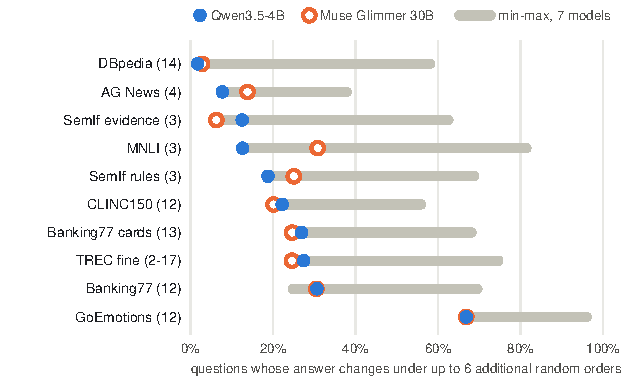
\includegraphics[width=\columnwidth]{figures/fig2-flips.pdf}
\caption{Share of questions whose answer changes under up to six additional random option orders, per source, ordered by Qwen 4B's rate. Option counts in parentheses. The band is the minimum to maximum over seven models.}
\label{fig:flips}
\end{figure}

\section{ChaosNLI}
\label{app:chaos}
Figure~\ref{fig:jsd} and Table~\ref{tab:chaos} give the ChaosNLI results per model. Averaging reduces the Jensen--Shannon divergence from the 100-annotator distribution on every model (Table~\ref{tab:models}). The mean divergence of the budget's single orders is within 0.01 bits of the base order's on every model, and the averaged distribution improves on it by 6 to 41\%. The target is the whole vote distribution, which reduces the dependence on a single gold label without removing annotation error \citep{webergenzel2024varierr}. Neither the averaged confidence nor the flip predicts a contested item (majority label under 60\% of votes). On items where at least 80 of 100 annotators chose the gold label, the confident flips of Qwen 2B and Muse 30B are wrong far more often than their stable confident answers; Granite Tiny and SmolLM3 show smaller contrasts; Qwen 4B has five flips there; Granite 3B and gpt-oss, weak on MNLI, show none.

\begin{figure}[t]
\centering
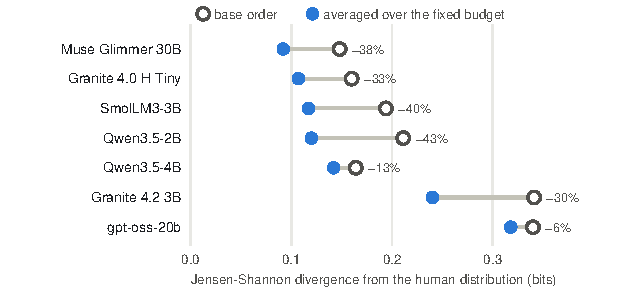
\includegraphics[width=\columnwidth]{figures/fig3-jsd.pdf}
\caption{Jensen--Shannon divergence from the human label distribution on ChaosNLI's 1,599 MNLI items, the base order compared with the average over the fixed budget.}
\label{fig:jsd}
\end{figure}

\begin{table*}[t]
\centering\footnotesize
\begin{tabular}{@{}lrrrrr@{}}
\toprule
 & MNLI wrong & Changing: wrong & Stable: wrong & AUROC, flip & AUROC, averaged conf. \\
\midrule
Qwen 4B & 17.1\% & 2/5 (40\%) & 8/140 (6\%) & 0.51 & 0.55 \\
Muse 30B & 20.1\% & 7/17 (41\%) & 3/90 (3\%) & 0.57 & 0.58 \\
gpt-oss 20B & 51.6\% & 14/19 (74\%) & 138/192 (72\%) & 0.48 & 0.48 \\
Granite 3B & 54.4\% & 81/132 (61\%) & 57/103 (55\%) & 0.46 & 0.46 \\
Granite Tiny & 34.8\% & 4/24 (17\%) & 8/78 (10\%) & 0.54 & 0.57 \\
SmolLM3 3B & 48.9\% & 7/58 (12\%) & 2/28 (7\%) & 0.52 & 0.56 \\
Qwen 2B & 43.0\% & 20/51 (39\%) & 5/29 (17\%) & 0.51 & 0.52 \\
\bottomrule
\end{tabular}

\caption{ChaosNLI, per model: confident answers (base-order confidence 0.9 or more) on items with at least 80\% annotator agreement, wrong among those that change under the fixed budget and among those that do not; each model's wrong-answer rate on the main run's 1,000 MNLI questions; AUROC for a contested item from the flip and from the averaged confidence. Granite 3B and gpt-oss are weak on MNLI (45.6\% and 48.4\% accuracy).}
\label{tab:chaos}
\end{table*}

\section{Every signal, both error targets}
\label{app:signals}
Table~\ref{tab:signals} scores every signal on both error targets, and Figure~\ref{fig:h1} shows the two central comparisons. For a wrong base-order answer the averaged confidence beats the base-order confidence by 0.01 to 0.06 AUROC; for a wrong averaged answer, by 0.02 to 0.10. Adding the spread to the averaged margin instead of the averaged confidence changes AUROC by $-0.008$ (Granite Tiny) to $+0.006$ (Granite 3B). The share of orders that change the answer, the coarser statistic, has AUROC 0.73 to 0.83 alone.

\begin{figure}[t]
\centering
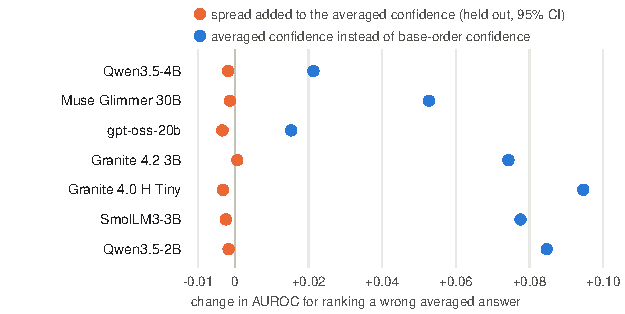
\includegraphics[width=\columnwidth]{figures/fig4-h1.pdf}
\caption{Change in AUROC for ranking a wrong averaged answer. Orange: adding the spread across orders to the averaged confidence, fitted leave-one-source-out, with 95\% bootstrap intervals; blue: the direct difference between the averaged confidence's AUROC and the base-order confidence's.}
\label{fig:h1}
\end{figure}

\begin{table*}[t]
\centering\footnotesize\setlength{\tabcolsep}{3pt}
\begin{tabular}{@{}lrrrrrrr@{}}
\toprule
 & Qwen 4B & Muse 30B & gpt-oss 20B & Granite 3B & Granite Tiny & SmolLM3 3B & Qwen 2B \\
\midrule
\multicolumn{8}{@{}l}{AUROC for a wrong base-order answer} \\
\quad base-order confidence & 0.863 & 0.832 & 0.836 & 0.755 & 0.787 & 0.804 & 0.799 \\
\quad averaged confidence & 0.880 & 0.875 & 0.847 & 0.811 & 0.839 & 0.844 & 0.839 \\
\quad spread & 0.866 & 0.867 & 0.832 & 0.809 & 0.815 & 0.827 & 0.825 \\
\quad flip & 0.777 & 0.797 & 0.731 & 0.764 & 0.820 & 0.825 & 0.818 \\
\quad candidate mass & 0.828 & 0.540 & 0.792 & 0.566 & 0.679 & 0.741 & 0.725 \\
\quad spread added, held-out gain & $-0.0017$ & $+0.0002$ & $-0.0040$ & $+0.0020$ & $-0.0031$ & $-0.0012$ & $+0.0001$ \\
\quad flip added, held-out gain & $+0.0035$ & $+0.0287$ & $+0.0340$ & $+0.2088$ & $+0.0757$ & $+0.0605$ & $+0.0572$ \\
\multicolumn{8}{@{}l}{AUROC for a wrong averaged answer} \\
\quad base-order confidence & 0.846 & 0.809 & 0.823 & 0.712 & 0.730 & 0.740 & 0.738 \\
\quad averaged confidence & 0.867 & 0.862 & 0.838 & 0.786 & 0.825 & 0.818 & 0.823 \\
\quad spread & 0.849 & 0.849 & 0.818 & 0.782 & 0.784 & 0.788 & 0.800 \\
\quad spread added, held-out gain & $-0.0018$ & $-0.0013$ & $-0.0034$ & $+0.0007$ & $-0.0032$ & $-0.0024$ & $-0.0017$ \\
\quad flip added, held-out gain & $+0.0035$ & $-0.0017$ & $-0.0047$ & $-0.0086$ & $-0.0019$ & $-0.0051$ & $-0.0013$ \\
\midrule
Answers at base-order confidence $\ge 0.9$ & 65\% & 45\% & 78\% & 86\% & 60\% & 53\% & 48\% \\
\quad of which changing under some order & 4\% & 4\% & 15\% & 37\% & 43\% & 31\% & 33\% \\
\quad wrong when changing & 27.4\% & 30.4\% & 41.7\% & 51.3\% & 34.5\% & 34.8\% & 29.1\% \\
\quad wrong when stable & 5.5\% & 3.5\% & 11.9\% & 13.6\% & 6.3\% & 6.8\% & 5.5\% \\
\quad wrong, all confident answers & 6.3\% & 4.5\% & 16.4\% & 27.4\% & 18.6\% & 15.3\% & 13.2\% \\
Adjusted odds ratio & 3.39 & 5.87 & 3.06 & 2.83 & 5.72 & 5.09 & 4.23 \\
Adjusted risk difference & $+0.094$ & $+0.114$ & $+0.121$ & $+0.160$ & $+0.210$ & $+0.195$ & $+0.132$ \\
Mantel--Haenszel odds ratio & 3.84 & 4.69 & 2.79 & 2.46 & 6.13 & 4.97 & 4.19 \\
\quad 95\% interval & 2.52--5.85 & 2.73--8.06 & 2.26--3.44 & 2.10--2.87 & 4.86--7.72 & 3.94--6.27 & 3.22--5.45 \\
\bottomrule
\end{tabular}

\caption{Error ranking by every signal on both error targets, and the confident subgroup (base-order confidence 0.9 or more), fixed budget, 6,944 questions per model. Held-out gains are AUROC differences of a leave-one-source-out logistic combination over the confidence alone.}
\label{tab:signals}
\end{table*}

\section{Flip robustness}
\label{app:robust}

\paragraph{Per source.} Table~\ref{tab:persource} gives the per-source odds ratios. On the sources with cleaner labels (CLINC150, MNLI, DBpedia, SemIf, AG News) Qwen 4B's Mantel--Haenszel odds ratio is 6.65, compared with 3.17 on the noisier four (Banking77 twice, GoEmotions, TREC). Leaving MNLI out raises Granite 3B's adjusted odds ratio from 2.83 to 4.63. The two MNLI exceptions are weak model-task pairs, not models guessing everywhere: their MNLI flip rates are 50\% and 28\%, so the cause of the reversal is not established.

\begin{table*}[t]
\centering\scriptsize\setlength{\tabcolsep}{3pt}
\begin{tabular}{@{}lrrrrrrr@{}}
\toprule
Source & Qwen 4B & Muse 30B & gpt-oss 20B & Granite 3B & Granite Tiny & SmolLM3 3B & Qwen 2B \\
\midrule
DBpedia & -- & -- & 1.9 (24)$^{\dagger}$ & 14.6 (61) & 16.2 (419) & 8.1 (168) & 8.0 (152) \\
AG News & -- & -- & 4.2 (58) & 3.2 (230) & 4.7 (186) & 7.8 (67) & 2.4 (188) \\
MNLI & 7.1 (10) & 10.3 (48) & 0.8 (106)$^{\dagger}$ & 0.6 (403) & 3.1 (81) & 3.1 (187) & 3.1 (244) \\
SemIf evidence & -- & -- & 5.7 (15)$^{\dagger}$ & -- (24) & -- & -- & -- (11) \\
SemIf rules & -- & -- & 2.2 (11)$^{\dagger}$ & -- (23) & -- & -- & -- \\
CLINC150 & 8.8 (34) & 21.2 (10) & 9.8 (124) & 10.9 (247) & 17.6 (273) & 15.9 (200) & 6.1 (117) \\
TREC fine & 4.8 (33) & -- & 4.0 (117) & 3.9 (218) & 2.7 (125) & 5.3 (73) & -- (87) \\
Banking77 cards & 4.9 (26) & -- (10) & 4.6 (86) & 4.9 (136) & 7.2 (169) & 7.7 (105) & 8.9 (50) \\
Banking77 & 2.1 (45)$^{\dagger}$ & 5.3 (22) & 6.7 (135) & 4.8 (306) & 7.4 (283) & 3.4 (172) & 5.7 (122) \\
GoEmotions & 3.0 (18) & 1.1 (14)$^{\dagger}$ & 2.3 (147) & 2.6 (545) & 3.9 (261) & 2.0 (139) & 3.9 (111) \\
\bottomrule
\end{tabular}

\caption{Per-source Mantel--Haenszel odds ratio for error among changing versus stable confident answers, stratified by confidence decile, with the number of confident flips in parentheses. $\dagger$: 95\% interval includes 1. A dash: fewer than ten flips or no estimable ratio.}
\label{tab:persource}
\end{table*}

\paragraph{Criterion paraphrases.} Each question of the eight public sources was also asked in the base order under three hand-written paraphrases of its criterion (6,848 questions). Reordering changes the answer on 24\% of questions and paraphrasing on 10\%; among confident answers, 171 change under order and 17 under paraphrase. Across all answers, the largest high-error subgroup is answers that survive every paraphrase and change under an order: 1,092 of them, 54\% wrong, compared with 9\% for answers stable under both. The budgets are unequal (six reorderings versus three paraphrases) and the paraphrases are hand-written, so this does not isolate the representation as the cause. It shows that the order flag is not the wording sensitivity these paraphrases elicit under a smaller budget.

\paragraph{Generated text, Qwen 4B.} Qwen 4B generated its answer for the same 6,944 questions in the same fixed budget, with two prompts: llav's own, and one that asks for the letter and the option's description. Decoding was greedy with 32 tokens and reasoning disabled, and the answer was parsed from the text. The generated answer equals the first-token argmax of the same call in 100\% of cases and llav's separate readout in 99.2\% (95.1\% with the longer-answer prompt). \citet{wang2024myanswer} report the mismatch persisting as prompts constrain the answer to a letter; it does not appear for this model with reasoning disabled.

Generated answers change under some order on 24 to 26\% of questions, compared with 24\% for the readout. A generated answer that changes is wrong 60\% of the time, versus 10\% for one that does not. Majority vote over the orders removes 7\% of generated errors, compared with 8\% for readout averaging. Generation took 61 and 118 minutes, compared with 95 minutes for the readout over about three times as many orders.

\paragraph{Hand audit.} A coding of Qwen 4B's 57 confident flipped errors (any-order flag) by two raters agreed on only half the codes (Cohen's $\kappa$ 0.23) and is not used as evidence. Averaging fixes 3 of those 57. A pilot that used each dataset's own option order as the reference showed a 41\% error rate among confident flips versus 4\% for stable ones; the randomized base order used here gives the estimates in the paper.

\section{PriDe}
\label{app:pride}
PriDe estimates the prior over option ids as the geometric mean of the observed id probabilities across a question's cyclic rotations, averaged over a sample, and divides it out of the others' base-order distributions \citep{zheng2024robust}. Five models were run in every cyclic rotation of questions with up to 14 options; the runner caps rotations at 13, so TREC's 94 seventeen-option questions drop out. A 5\% sample per source and option count estimates the prior, and the remaining 6,508 questions are evaluated, with the fixed-budget average on the same questions as the comparison. Wrong answers, base / PriDe / averaged: Qwen 4B 21.7 / 23.0 / 20.0\%; Qwen 2B 34.5 / 30.3 / 28.6\%; Granite 3B 32.8 / 32.1 / 29.2\%; Granite Tiny 34.5 / 32.6 / 27.4\%; SmolLM3 35.8 / 34.3 / 30.5\%.

PriDe's degradation on Qwen 4B appears to come from its estimate of the prior for position A. The model's decisions are position-neutral: on AG News the argmax lands on positions A to D 26, 25, 25 and 25\% of the time. But position A is almost never given a tiny probability (below 0.001 in 16\% of rotations, versus 49 to 57\% for the others). PriDe's log-space estimator reads that floor as a prior of 0.73 on A and divides it out, pushing decisions toward later positions. The letter bias of this readout sits in the tail of the distribution where it does not affect decisions; a multiplicative correction moves the decisions anyway. Qwen 2B has decision-level position bias (MNLI argmax share 0.54, 0.33, 0.13 by position), and there PriDe does help, though less than averaging.

\section{Cost}
\label{app:cost}
Table~\ref{tab:cost} gives the timings. Asking in $K$ orders costs $K$ suffix decodes over one shared prefix. A first request, which also reads the 1,800-token state, takes about 0.30~s, 0.25~s more than the cached repeat. The batching in llav's native helper removes the per-pass overhead, not the decode of each suffix; \citet{guda2025rethinking} report the same construction and the same linearity.

\begin{table}[t]
\centering\small
\begin{tabular}{@{}rrr@{}}
\toprule
Orders $K$ & Batched helper & llama-server \\
\midrule
1 & 46 ms & 62 ms \\
2 & 69 ms & 110 ms \\
4 & 121 ms & 208 ms \\
7 & 192 ms & 354 ms \\
14 & 420 ms & 697 ms \\
\bottomrule
\end{tabular}
\caption{Per-question latency for $K$ orders of a 7-option question with a cached 1,800-token state (median of 8 repeats, RTX PRO 4000, Qwen3.5-4B Q8\_0).}
\label{tab:cost}
\end{table}

\section{Candidate mass}
\label{app:mass}
The runtime reports the probability mass assigned to the option letters, meant to flag questions none of the options fit. As an error signal it is the weakest (Table~\ref{tab:signals}). Removing the gold option from 1,400 questions and asking again moves the median mass only from 0.9998 to 0.9991, and 4.9\% of the cut questions fall below the runtime's 0.9 cue, compared with 0.07\% of the full ones. Candidate mass therefore does not detect a missing correct answer when the remaining options are plausible; its behaviour when no option is plausible remains unmeasured.

\section{Reproduction}
\label{app:repro}
\texttt{scripts/evaluate.py fetch} downloads the sources. \texttt{scripts/perturb.py run} asks a running llav each question in the orders described; \texttt{analyze} reports the noise floor, the signal AUROCs, the spread and flip tests and the paired intervals; \texttt{h2} the adjusted flip effect; \texttt{human} the ChaosNLI analyses; \texttt{pride} the PriDe comparison; \texttt{text} the generated-text arm; \texttt{nofit} the candidate-mass pairs; and \texttt{run --reword} the paraphrase control. \texttt{paper/extract.py} collects every number in this paper from the raw result files into the committed \texttt{paper/data/summary.json}, from which \texttt{paper/tables.py} and \texttt{paper/figures.py} write the tables and figures.

\end{document}
